%%%%%%%%%%%%%%%%%%%%%%%%%%%%%%%%%%%%%%%%%%%%%%%%%%%%%%%%%%%%
%%  This Beamer template was created by Cameron Bracken.
%%  Anyone can freely use or modify it for any purpose
%%  without attribution.
%%
%%  Last Modified: January 9, 2009
%%

\documentclass[xcolor=x11names,compress, graphics]{beamer}
\usepackage{etex}
%% General document %%%%%%%%%%%%%%%%%%%%%%%%%%%%%%%%%%
\usepackage{graphicx}
\usepackage{tikz}
\usetikzlibrary{decorations.fractals}
%%%%%%%%%%%%%%%%%%%%%%%%%%%%%%%%%%%%%%%%%%%%%%%%%%%%%%
\usepackage{movie15}
\usepackage{float}
\usepackage{subfig}
\usepackage{amsmath}
\usepackage{amsfonts}
\usepackage{mathrsfs}
\usepackage{mathtools}

\usepackage{algorithm, algorithmic}

%% Beamer Layout %%%%%%%%%%%%%%%%%%%%%%%%%%%%%%%%%%
\useoutertheme[subsection=false,shadow]{miniframes}
\useinnertheme{default}
\usefonttheme{serif}
\usepackage{palatino}

\setbeamerfont{title like}{shape=\scshape}
\setbeamerfont{frametitle}{shape=\scshape}

\setbeamercolor*{lower separation line head}{bg=DeepSkyBlue4} 
\setbeamercolor*{normal text}{fg=black,bg=white} 
\setbeamercolor*{alerted text}{fg=red} 
\setbeamercolor*{example text}{fg=black} 
\setbeamercolor*{structure}{fg=black} 
 
\setbeamercolor*{palette tertiary}{fg=black,bg=black!10} 
\setbeamercolor*{palette secondary}{fg=black,bg=black!10}
\setbeamercolor*{palette quaternary}{fg=black,bg=black!10} 

%% Set the background and font color of the blocks 
\setbeamercolor{block title}{bg=DeepSkyBlue4,fg=white}

%% Set the type of the blocks
\setbeamertemplate{blocks}[shadow=true]

\newcommand{\topline}{%
  \tikz[remember picture,overlay] {%
    \draw[DeepSkyBlue4] ([yshift=-1.5cm, xshift = 1cm]current page.north west)
             -- ([yshift=-1.5cm,xshift=\paperwidth-1cm]current page.north west);}}
             
\setbeamertemplate{section in toc}[sections numbered]           

\renewcommand{\(}{\begin{columns}}
\renewcommand{\)}{\end{columns}}
\newcommand{\<}[1]{\begin{column}{#1}}
\renewcommand{\>}{\end{column}}

\usepackage[skip=10pt,font=scriptsize]{caption}
\captionsetup[figure]{labelformat=empty}

\DeclarePairedDelimiter\floor{\lfloor}{\rfloor}

\makeatother
\setbeamertemplate{footline}
{
  \leavevmode%
  \hbox{%
  \begin{beamercolorbox}[wd=.4\paperwidth,ht=2.25ex,dp=1ex,center]{author in head/foot}%
    \usebeamerfont{author in head/foot}\insertshortauthor
  \end{beamercolorbox}%
  \begin{beamercolorbox}[wd=.6\paperwidth,ht=2.25ex,dp=1ex,center]{title in head/foot}%
    \usebeamerfont{title in head/foot}\insertshorttitle\hspace*{3em}
    \insertframenumber{} / \inserttotalframenumber\hspace*{1ex}
  \end{beamercolorbox}}%
  \vskip0pt%
}
\makeatletter
%%%%%%%%%%%%%%%%%%%%%%%%%%%%%%%%%%%%%%%%%%%%%%%%%%

\title{\scshape \textbf{C Basics}}
\author{\scriptsize\scshape Angel No\'e Mart\'inez Gonz\'alez}


\usepackage{listings}

\begin{document}

% The title page
\begin{frame}
\setcounter{framenumber}{1}
\titlepage
\scriptsize

\end{frame}
%===============


\section[\scshape Composed Types]{\scshape Composed Types}
\begin{frame}[fragile,allowframebreaks ]{Composed Types}
\topline

{\Large\scshape Typedef Definitions}

\begin{lstlisting}[language=C++,basicstyle=\ttfamily,keywordstyle=\color{blue}]
typedef struct personStruct {
	unsigned int edad;
	unsigned int altura;
}persona;

persona angel, jorge;

\end{lstlisting}

\framebreak
\topline

{\Large\scshape Data Alignment}
\begin{figure}
	\begin{center}
		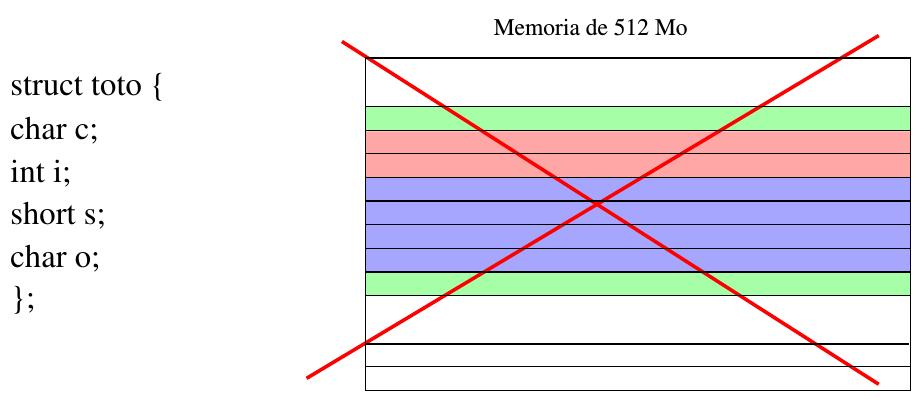
\includegraphics[width=10cm]{Figures/bad_alignment.jpg}
	\end{center}
\end{figure}

What's the size?

\framebreak
\topline

The compiler pads with extra bytes, but why?

\begin{figure}
	\begin{center}
		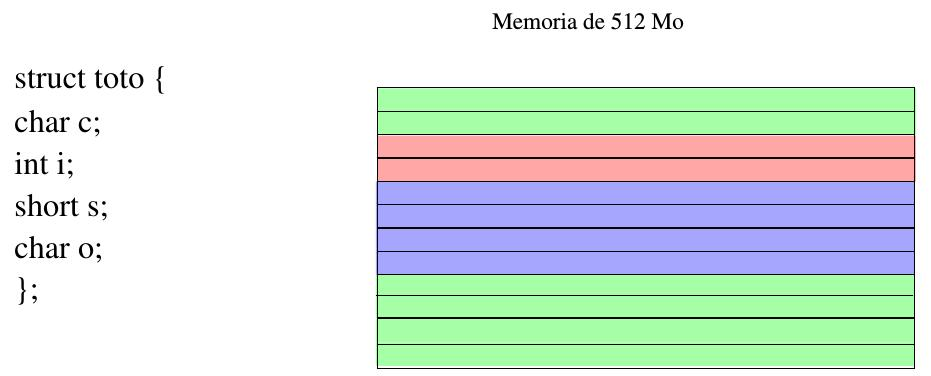
\includegraphics[width=10cm]{Figures/good_alignment.jpg}
	\end{center}
\end{figure}

The compiler adds extra data to align and to facilitate access.

\framebreak
\topline

The machine access to memory by buses of size depending on the granularity of the OS: 2, 4, 8 and 16 bytes.

\begin{figure}
	\begin{center}
		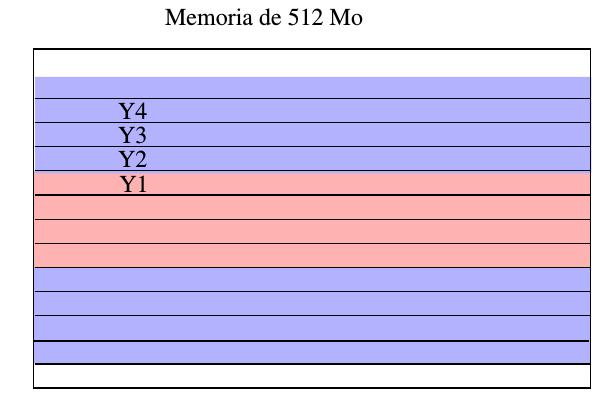
\includegraphics[width=7cm]{Figures/databuses.jpg}
	\end{center}
\end{figure}

Thinking the organization of data helps alignment. Can you think a best ordering in toto struct?

\end{frame}

\section[\scshape Pointers]{\scshape Pointers}
\begin{frame}[fragile,allowframebreaks ]{Pointers}
\topline

A pointer is a type that refers a data in memory, contains
\begin{itemize}
	\item Memory address
	\item The way to read data, i.e. data type.
	\item Access to the value example
	
\begin{lstlisting}[language=C++,basicstyle=\ttfamily,keywordstyle=\color{blue}]
int a=10;
int* a_ptr = &a;
*a_ptr = a*a;
a_ptr[0] = *a_ptr + 1;
\end{lstlisting}	

	\item Operator priority level
	
\begin{lstlisting}[language=C++,basicstyle=\ttfamily,keywordstyle=\color{blue}]
int a=10;
int* a_ptr = &a;
int c = a**b**b;
printf("%d", c);
\end{lstlisting}	

	\item Composed types pointers
	
\begin{lstlisting}[language=C++,basicstyle=\ttfamily,keywordstyle=\color{blue}]
person jorge;
person* jorge_ptr=&jorge;
jorge_ptr->edad = 30;
(*jorge_ptr).edad = 30;
\end{lstlisting}	

\end{itemize}


\framebreak
\topline

Arithmetic: a pointer is an integer, we can then

\begin{itemize}
	\item Add an integer to a pointer, which result a translated pointer in memory.
	\item Subtract an integer to a pointer, which result a translated pointer in memory.
	\item Subtract a pointer to a pointer, which result in the memory between these pointers.
\end{itemize}

All these results are given in units corresponding to the data of the pointers not just bytes.


\framebreak
\topline

When data structures are too big it can be very costly to pass variables to functions (it will copy). We can then pass the address of the variable to avoid data to be copied.

{\scriptsize
\begin{lstlisting}[language=C++,basicstyle=\ttfamily,keywordstyle=\color{blue}]
typedef struct{
	int dummy;
	...
} MyBigData;

void my_usage_func(MyBigData* data) { 
	// Some code
	data->dummy;
}


MyBigData data;

my_usage_func(&data);
\end{lstlisting}	
}

\framebreak
\topline


{\Large\scshape Double Pointers}: a pointer has a given type, has a value stored in memory then we can define a pointer to a pointer

\begin{lstlisting}[language=C++,basicstyle=\ttfamily,keywordstyle=\color{blue}]
int a=10;
int* a_ptr=&a;
int** a_ptr_ptr = &a_ptr;
\end{lstlisting}	


\framebreak
\topline

{\Large\scshape Pointers of Functions}

\end{frame}

\section[\scshape Allocation]{\scshape Allocation}
\begin{frame}[fragile,allowframebreaks ]{Memory Allocation}
\topline


A dynamic array survives outside the function call. Function malloc takes as parameter the number of bytes to be allocated and return a void *

\begin{lstlisting}[language=C++,basicstyle=\ttfamily,keywordstyle=\color{blue}]
int* myarray 
      = (int*)malloc(sizeof(int)*sizeOfMyArray);
\end{lstlisting}	

we need to cast the return value to the data type of our array. There is not initialization value for the arrays.

\framebreak
\topline

The function calloc does initialize the values to 0.

\begin{lstlisting}[language=C++,basicstyle=\ttfamily,keywordstyle=\color{blue}]
int* myarray 
      = (int*)calloc(sizeof(int)*sizeOfMyArray);
\end{lstlisting}	

\framebreak
\topline

We need to be sure that our memory request was succesfull, on the other case malloc and calloc returns NULL

\begin{lstlisting}[language=C++,basicstyle=\ttfamily,keywordstyle=\color{blue}]
int* myarray 
      = (int*)calloc(sizeof(int)*sizeOfMyArray);
      
if(myarray==NULL)
	// Do something to manage the error
\end{lstlisting}	

\framebreak
\topline

{\Large\scshape Multiple dynamic arrays}

\begin{lstlisting}[language=C++,basicstyle=\ttfamily,keywordstyle=\color{blue}]

int** mydoublePointerArray = 
      (int**)malloc(sizeof(int*)*myFirstDimentionSize);
int i;
for(i=0; i<myFirstDimentionSize; i++)
    mydoublePointerArray[i] = (int*)malloc(sizeof(int)*mySecondDimentioinSize);
mydoublePointerArray[x][y] = z;
// Some code
for(i=0; i<myFirstDimentionSize; i++)
    if(mydoublePointerArray[i]!=NULL)
        free(mydoublePointerArray[i])

if(mydoublePointerArray!=NULL)
    free(mydoublePointerArray);
\end{lstlisting}

Always verify if the array points to some valid memory location.



\framebreak
\topline

Once we have finished using the memory, we need to return it to the system

\begin{lstlisting}[language=C++,basicstyle=\ttfamily,keywordstyle=\color{blue}]

if(myarray!=NULL)
    free(myarray)

\end{lstlisting}

Always verify if the array points to some valid memory location.


\end{frame}

\end{document}